\section{Análise do Cenário PitchRoll}

Neste cenário, o quadricóptero foi submetido a um comando de pitch seguido de um comando de roll, onde avaliamos as respostas nas coordenadas de arfagem, guinada, rolagem e nas coordenadas \(x\), \(y\) e \(z\).

\subsection{Arfagem}

\begin{figure}[H]
    \centering
    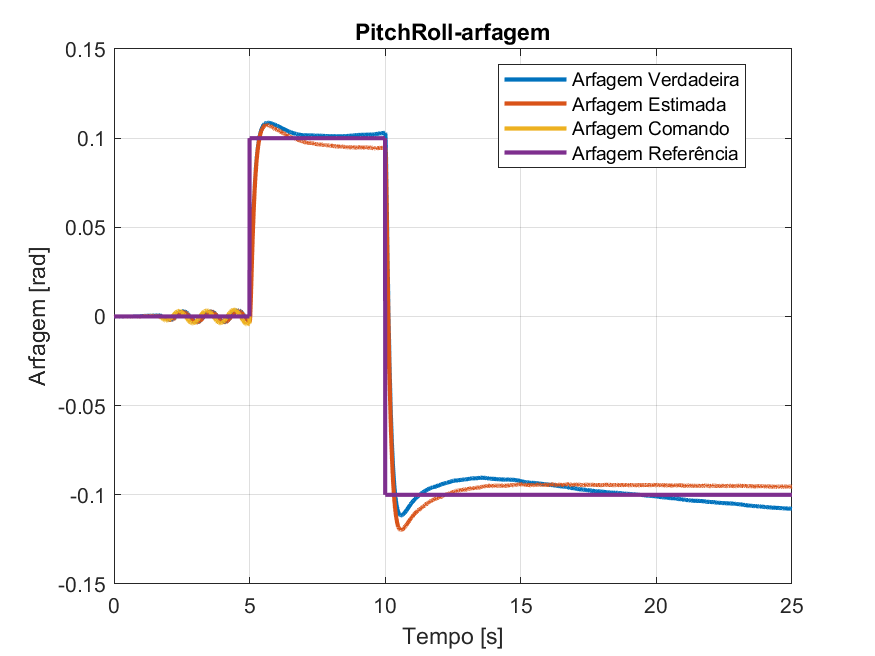
\includegraphics[width=0.7\textwidth]{PitchRoll-arfagem.png}
    \caption{Resposta em Arfagem para o cenário Pitch seguido de Roll}
    \label{fig:pitchroll-arfagem}
\end{figure}

No gráfico da Figura \ref{fig:pitchroll-arfagem}, observamos que, após o comando inicial de pitch, o sistema rapidamente se ajusta, mas, ao adicionar o comando de roll, ocorre uma oscilação significativa. Esse comportamento sugere uma leve instabilidade momentânea ao alternar entre os dois comandos. A diferença entre a curva estimada e a verdadeira também se torna mais evidente após o comando de roll, indicando a necessidade de ajustes nos parâmetros do controlador para uma resposta mais uniforme e próxima da referência.

\subsection{Guinada}

\begin{figure}[H]
    \centering
    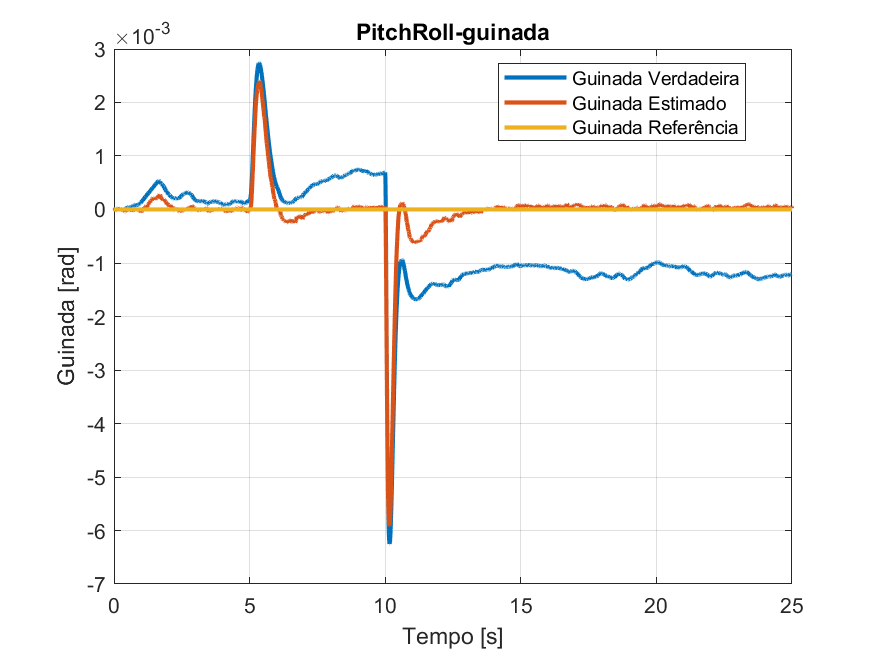
\includegraphics[width=0.7\textwidth]{PitchRoll-guinada.png}
    \caption{Resposta em Guinada para o cenário Pitch seguido de Roll}
    \label{fig:pitchroll-guinada}
\end{figure}

Na Figura \ref{fig:pitchroll-guinada}, notamos uma oscilação acentuada na guinada, especialmente após o comando de roll. A curva verdadeira apresenta uma amplitude significativamente maior do que a curva estimada, o que indica que o controlador está tendo dificuldade em amortecer as oscilações na guinada durante as mudanças de atitude. Isso sugere que o sistema pode estar subamortecido para este eixo, e um aumento no ganho derivativo pode ajudar a reduzir essa instabilidade.

\subsection{Rolagem}

\begin{figure}[H]
    \centering
    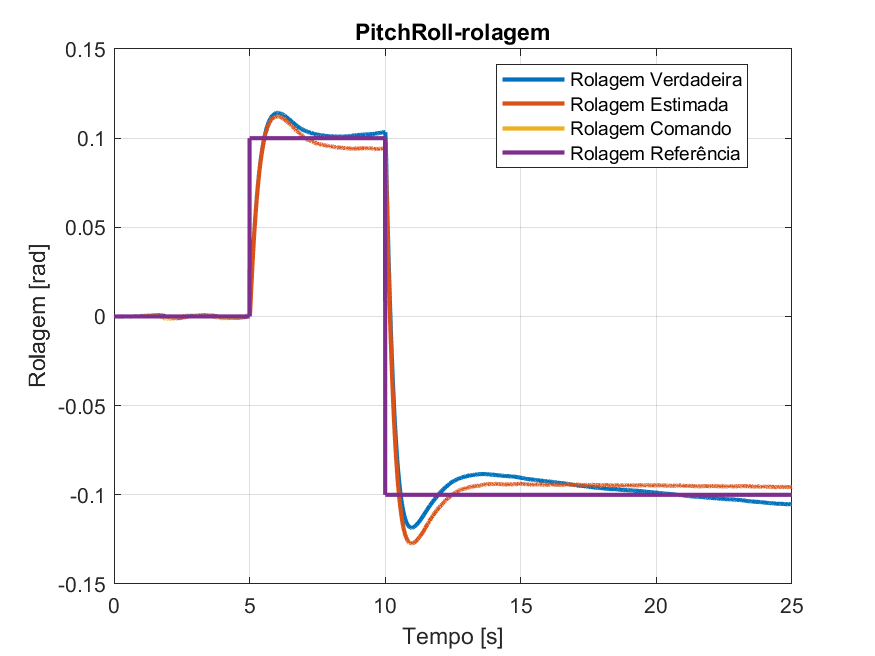
\includegraphics[width=0.7\textwidth]{PitchRoll-rolagem.png}
    \caption{Resposta em Rolagem para o cenário Pitch seguido de Roll}
    \label{fig:pitchroll-rolagem}
\end{figure}

A Figura \ref{fig:pitchroll-rolagem} mostra que, com a introdução do comando de roll, a resposta do sistema apresenta uma oscilação rápida e estabiliza, embora com uma leve diferença entre o valor verdadeiro e o estimado. A resposta geral sugere que o controlador de rolagem é eficaz em manter o controle, mas ajustes finos podem melhorar a precisão entre a resposta verdadeira e a estimada.

\subsection{Coordenadas X, Y e Z}

\begin{figure}[H]
    \centering
    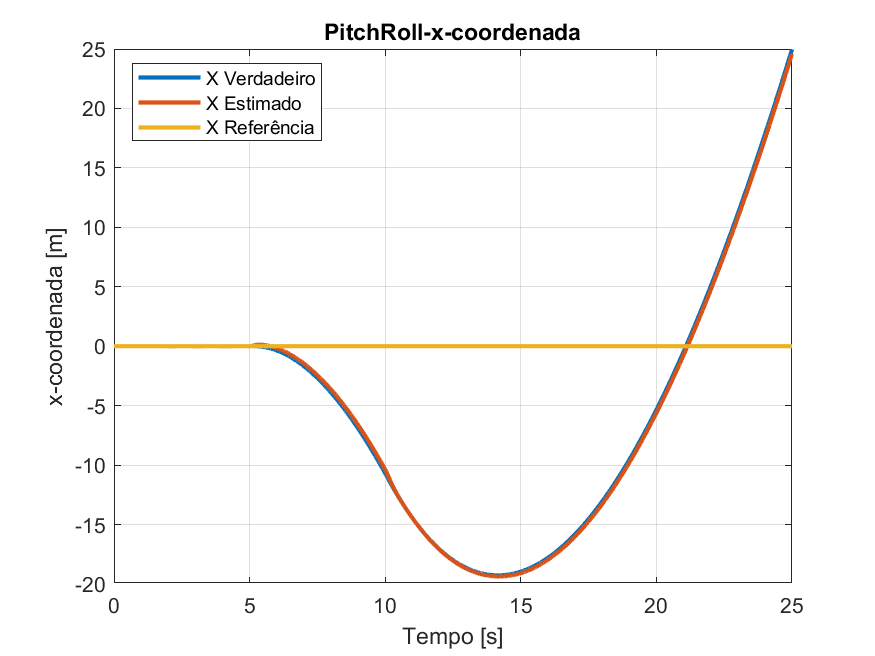
\includegraphics[width=0.45\textwidth]{PitchRoll-x-coordenada.png}
    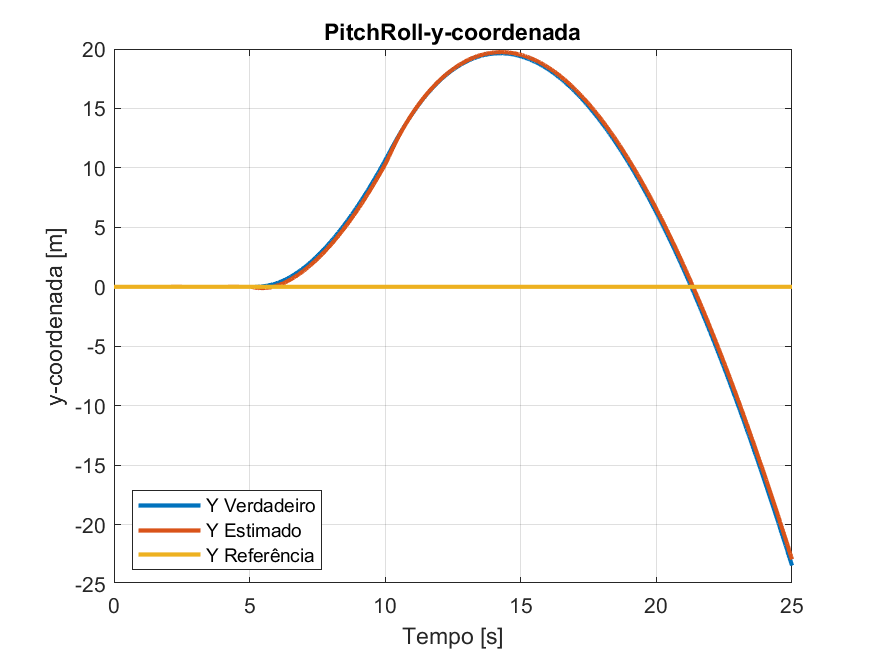
\includegraphics[width=0.45\textwidth]{PitchRoll-y-coordenada.png}
    \caption{Resposta nas coordenadas X e Y para o cenário Pitch seguido de Roll}
    \label{fig:pitchroll-xy-coordenadas}
\end{figure}

Nas Figuras \ref{fig:pitchroll-xy-coordenadas}, observamos que as coordenadas \(x\) e \(y\) sofrem uma mudança significativa, especialmente no eixo \(x\), onde o quadricóptero apresenta um movimento de deslocamento contínuo, o que reflete o impacto dos comandos de pitch e roll. A trajetória estimada acompanha a verdadeira, mas com um pequeno desvio. Esses desvios indicam que a estimativa de posição do sistema de controle precisa de ajustes para rastrear com maior precisão.

\begin{figure}[H]
    \centering
    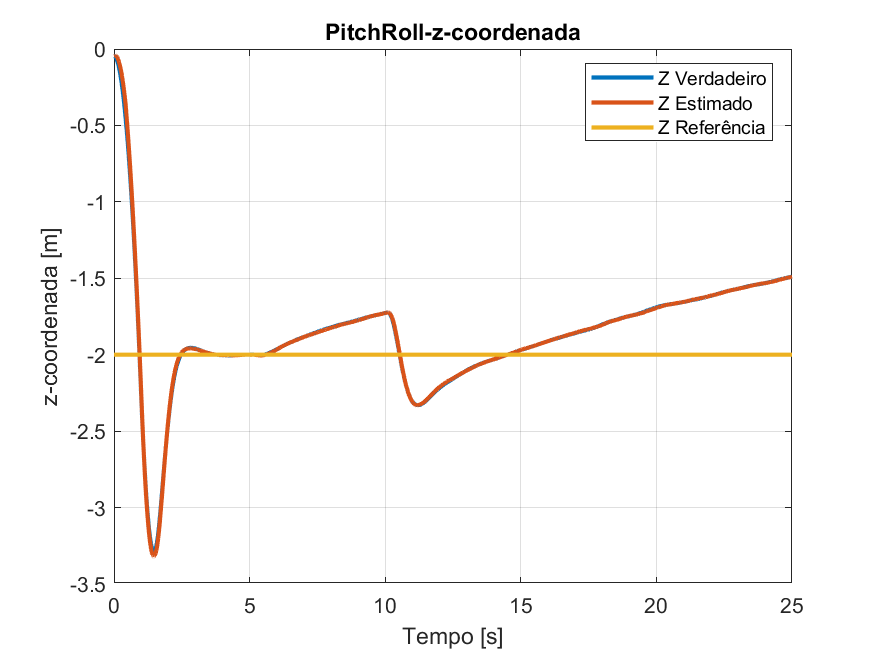
\includegraphics[width=0.7\textwidth]{PitchRoll-z-coordenada.png}
    \caption{Resposta na coordenada Z para o cenário Pitch seguido de Roll}
    \label{fig:pitchroll-z-coordenada}
\end{figure}

Na Figura \ref{fig:pitchroll-z-coordenada}, a coordenada \(z\) apresenta uma leve oscilação após os comandos de pitch e roll, com uma tendência de subir ligeiramente após o segundo comando. Este comportamento indica que o controlador de altitude está reagindo aos comandos de pitch e roll com uma pequena alteração na altitude. Ajustes no controlador de altitude podem ser necessários para minimizar o impacto dessas oscilações.

%\subsection{Conclusão do Cenário PitchRoll}

%O cenário Pitch seguido de Roll evidencia que o sistema responde bem a comandos individuais de pitch e roll, mas apresenta desafios ao lidar com ambos simultaneamente, especialmente em relação à guinada e à estabilidade nas coordenadas \(x\) e \(y\). O controlador poderia ser aprimorado para lidar melhor com a combinação de comandos e minimizar o impacto em outros eixos, garantindo uma maior estabilidade e precisão.


%---------------------------------------------------------------------
% INDICE REMISSIVO
%---------------------------------------------------------------------
\phantompart
\printindex
%---------------------------------------------------------------------
